\section{Detection and Time Synchronization}
\label{sec:detection}

As illustrated in Figure~\ref{fig:sig_acquis_chain}, the first step to analyze
the signal acquisition chain is to formulate the detector.
The detection algorithm proceeds sequentially and each step a window of length $N$ received samples with 
$N{-}1$ overlapped samples from the previous window is considered. The sequential detection problem solved 
in this paper is fundamentally equivalent to sequential frame synchronization~\cite{Massey_72,Lui_Tan_86,Scholtz_80}.
To make analysis easier, we focus on deriving the detection algorithm   
by assuming the fractional delay $\Delta p$ in~\eqref{eq:model} is neglected at a sufficiently high sample rate.
The effect of $\Delta p$ on our propose detection algorithm will be simulated with different sampling rate, 
or equivalently, different oversampling factor $M$ in Section~\ref{sec:simulations}. 

\begin{figure}[t]
  \centerline{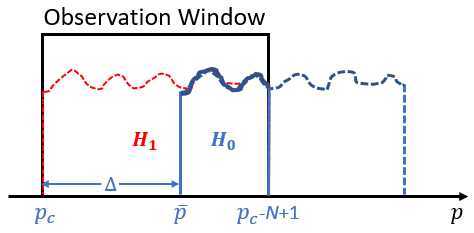
\includegraphics[width=2.4in]{H1_H0_hypothesis.png}}
  \caption{Received sequence in observation window (the shaded area) containing partial preamble (Blue: current received sequence; Red: received sequence at true delay $\bar{p}$. The noise level is omitted)}
  \label{fig:H1_H0_hypothesis}
  \end{figure}

We start by looking at the likelihood ratio test (LRT) for the detection task:
Let $H_0$ be the null hypothesis that the preamble is not completely presented in the received sequence from the obeservation window 
against the alternative $H_1$ that it does. 
Define $\Delta$ to be the distance between current received sequence at position $p_c$ and the true position ($\bar{p}$) of the preamble, 
i.e., $\Delta=|\bar{p}-p_c|$. Figure~\ref{fig:H1_H0_hypothesis} demonstrates the situation when received sequence containing the preamble has not completely passed the observation window.
It is symmetric if the partial preamble shows on the left side, i.e., has passed the observation window ($p_c>\bar{p}$).
It is obvious that under $H_0$, $\Delta \neq 0$ while $H_1$ means $\Delta=0$. 
Based on~\eqref{eq:model}, the conditional likelihood ratio test (LRT) can be built 
between $H_0$ and $H_1$ by giving the distance $\Delta$, the phasor $S{=}Ae^{j\phi}$ and frequency offset $b{=}e^{j2\pi \delta}$
at true delay $\bar{p}$,

\begin{equation}
  \label{eq:likelihood ratio}
  \begin{aligned}
  \Lambda(R|S,b,\Delta)=&~\frac{p_{R|H_1,S,b}(r|H_1,S,b)}{p_{R|H_0,S,b,\Delta}(r|H_0,S,b,\Delta)} \\
  =&~\frac{\displaystyle \prod_{n=0}^{N-1}\frac{1}{\sqrt{\pi N_0}}\exp{\bigg\{-\frac{1}{2}\frac{|r_{n}{-}s_nSb^n|^2}{N_0/2}\bigg\}}}{\displaystyle \prod_{n=\Delta}^{N-1} \frac{1}{\sqrt{\pi N_0}} \exp{\bigg\{-\frac{1}{2}\frac{|r_{n}{-}s_{n-\Delta}Sb^{n-\Delta}|^2}{N_0/2}\bigg\}}} ~\times \\
  &\quad~~~~~~~~~~~~~ \frac{1}{\displaystyle \prod_{n=0}^{\Delta-1} \frac{1}{\sqrt{\pi N_0}} \exp{\bigg\{-\frac{1}{2}\frac{|r_n|^2}{N_0/2}\bigg\}}} \LRT{H_1}{H_0} \eta.
  \end{aligned}
\end{equation}
Cancelling the common parts and taking the logarithm,~\eqref{eq:likelihood ratio} is reduced to

\begin{equation}
    \label{eq:log likelihood}
    \begin{aligned}
    \Re\Bigg\{\sum_{n=0}^{N-1}r_{n}s^*_nS^*b^{-n}-
    \sum_{n=\Delta}^{N-1}r_{n}s^*_{n-\Delta}S^*b^{-(n-\Delta)}\Bigg\}
    &\LRT{H_1}{H_0} \frac{N_0}{2}\ln\eta \\
    &+\frac{A^2}{2}\sum_{n=N-\Delta}^{N-1}|s_n|^2.
    \end{aligned}
\end{equation}
The second summation on the left hand side of~\eqref{eq:log likelihood} points to the inner product of the overlap between
the observed (partial) preamble and the true preamble. 
Or, to put it another way,~\eqref{eq:log likelihood} says that the log-likelihood 
ratio test equals to the difference between full cross-correlation and overlapped cross-correlation
between received and reference sequences. 
However, note that in practice, the latter cannot be
precomputed during detection process since $\Delta$ is an unknown information to the receiver.
One way to solving this problem is to simply move the overlapped cross-correlation to the right hand side  and
let it be reflected by the threshold.
Thus, based on the above discussion, after some proper scaling, the LRT finally reduces to a generalized correlation function in terms of the time instant (delay) $p$,

\begin{equation}
    \label{eq:generalized_corr}
    \rho(p)=
    \frac{\Re\{\langle
      \bm{r}_{p},\hat{\bm{s}}_{p}\rangle\}}
    {||\bm{r}_{p}||\cdot||\hat{\bm{s}}_{p}||} \LRT{H_1}{H_0} \gamma
  \end{equation}
where $\hat{\bm{s}}_{p}$ denotes the carrier-estimate corrected preamble, i.e., $\hat{s}_{p}[n]~{=}~s_{n}\hat{S}_{p}\hat{b}_{p}^n$ for $n=0,\ldots,N{-}1$,
at delay $p_c$. $\hat{b}_{p_c}$ and $\hat{S}_{p_c}$ are the frequency and phasor estimates at delay $p_c$.
$||\bm{r}_{p}||$ is the Euclidean norm of the received signal at delay $p$.
$\gamma$ is the normalized detection threshold which lies on the range of $[0,1]$.
Note, the LRT in~\eqref{eq:likelihood ratio} is not practical since the frequency and phasor offsets at true delay $\bar{p}$
is unknown while detection as well as the distance $\Delta$. 
Thus, instead of LRT, a generalized likelihood ratio test (GLRT) based detector is built relying on frequency and phasor estimates from each window of received sequence;
To get $\hat{b}_{p_c}$ and $\hat{S}_{p_c}$,
recall the LRT of~\eqref{eq:likelihood ratio} is built conditionally on the known frequency and phase offset 
at the true position $\bar{p}$ of the preamble; Therefore, the algorithm of computing the frequency and phase estimates at $p_c$ 
can be also derived by assuming the current received sequence contains the complete preamble.
% this tells the reason why we do estimation by assuming the position of preamble is known.

In conclusion, a GLRT based detector in~\eqref{eq:generalized_corr} is derived for detection task in this paper, and it relies on the frequency and phase estimates of the observed data sequence.
Furthermore, since the sequential detection proceeds at every time instant, 
to make it work at high sampling rate, 
the complexity of designed estimator for building~\eqref{eq:generalized_corr} becomes
much crucial. An estimator with very low 
computational complexity should be derived for real detection purpose.

% should not include the original fractional delay part since I don't know the meaning for introducing the expected loss.
% I think to talk about how large of the oversampling factor that the effect of fractional delay can be neglected is meaningful but not deep.







